% CS F407 Artificial Intelligence: final project report.
% Adapted to the supplied Project_Sub_Template format.
\documentclass[11pt,a4paper,twocolumn]{article}

\usepackage[margin=2cm,columnsep=0.8cm]{geometry}
\usepackage[T1]{fontenc}
\usepackage{lmodern}
\usepackage{microtype}
\usepackage{amsmath,amssymb}
\usepackage{graphicx}
\usepackage{booktabs}
\usepackage{tabularx}
\usepackage{enumitem}
\usepackage{titlesec}
\usepackage[hidelinks]{hyperref}
\pdfmapfile{+lm.map}

\titleformat{\section}{\normalsize\bfseries}{\thesection}{0.6em}{}
\titlespacing*{\section}{0pt}{1.2ex plus 0.3ex}{0.6ex}
\setlist{nosep,leftmargin=*}
\setlength{\parskip}{0.3ex}

\newcommand{\teamno}{Team Chaoshawk}
\newcommand{\githuburl}{https://github.com/sbhilare343/chaoshawk}

\begin{document}

\twocolumn[{%
\begin{center}
  {\large\bfseries A Safety-Gated Chaos-Metric Supervisor for UAVs in Lorenz-Derived Disturbances}\\[1ex]
  \teamno\\
  \begin{minipage}{0.94\textwidth}
    \centering\small
    Shubham Bhilare (CSIS, PhD Student, 2026PHXP0022G)\\
    Kadapa Dileep Hussain (Mechanical Engineering, PhD Student, 2026PHXP0064G)\\
    Dr. Tirtharaj Dash (Assistant Professor, CSIS)\\[0.5ex]
    BITS Pilani, K. K. Birla Goa Campus
  \end{minipage}\\[1.5ex]
  \begin{minipage}{0.85\textwidth}
    \small
    \centerline{\bfseries Abstract}\vspace{0.5ex}
    Small unmanned aerial vehicles can become difficult to supervise when an
    external disturbance changes faster than a human operator can interpret
    individual sensor readings. This project develops a software boundary that
    turns acceleration-like telemetry into a bounded instability indicator and
    uses that signal to choose conservative, high-level strategies. The system
    combines a Lorenz disturbance generator, a causal acceleration and jerk
    metric, an offline Rosenstein-style Lyapunov estimator, deterministic safety
    gates, and an optional structured language-model proposal interface. A
    matched 35-second reference experiment with seed 7 reduced horizontal RMS
    error from 72.206 m to 21.839 m and maximum error from 99.972 m to 29.432 m.
    These results validate the reproducible data and decision pipeline, but not
    physical flight stability. The repository provides the paper, source code,
    tests, and instructions needed to repeat the experiment.
  \end{minipage}
\end{center}
\vspace{1.5ex}
}]

\section{Introduction}
An autonomous UAV has to react to disturbances while its flight controller
continues to satisfy basic safety constraints. A supervisory system can help by
compressing telemetry into a small number of interpretable signals and by
choosing a response before a large position error develops. The difficulty is
that a disturbance indicator is uncertain. It can be affected by sensor noise,
irregular timestamps, vehicle motion, and estimator behavior. It should
therefore inform a bounded policy, not directly control motors.

This project studies that design problem through a reproducible reference
backend and a corresponding ROS 2 and PX4 integration path. The input to the
offline system is a seeded Lorenz trajectory used as a disturbance. The output
is simulated position, velocity, altitude, telemetry, an instability trace, and
high-level strategy events. The live interface accepts PX4 odometry and IMU
messages and publishes a metric and, only in simulation, bounded position
setpoints.

The contributions are threefold. First, the project provides a causal,
bounded instability indicator and an offline largest-Lyapunov estimator with a
sampling-quality guard. Second, it places deterministic freshness and safety
checks after every optional language-model proposal. Third, it supplies a
matched-seed experiment, tests, plots, machine-readable metadata, and a paper
that can be reproduced from a public repository.

\section{Background and related work}
The Lorenz equations are a classic deterministic nonlinear system that can
produce sensitive, non-periodic trajectories~\cite{lorenz}. They are useful in
this project as a controlled source of repeatable variation. They are not a
claim that a UAV in the experiment is itself a Lorenz system. The generated
state is scaled to form a disturbance input for a simple reference model.

A Lyapunov exponent describes the average growth of nearby trajectories. The
Rosenstein method estimates the largest exponent from a scalar time series by
delay embedding, finding temporally separated neighbors, and fitting their
mean logarithmic separation~\cite{rosenstein}. In this project the estimate is
treated as a finite-window instability feature. The implementation explicitly
warns that noise, forcing, and inadequate sampling can produce a positive
value.

From an artificial intelligence perspective, the supervisory agent is a
constrained decision interface rather than an end-to-end learned controller.
The optional language model receives a structured observation and is asked to
return one of three strategy names with a timestamp. This resembles a tool-use
or function-calling interface, but the returned object is still untrusted. The
local validator is authoritative. This choice follows the general principle
that planning or reasoning components should be separated from execution
constraints~\cite{russell2021aima}. The current results do not evaluate an LLM
against the deterministic policy, since the reported runs use no API key.

\section{Method}
\subsection{Reference disturbance and vehicle update}
The disturbance is generated from
\begin{equation}
\dot{x}=\sigma(y-x),\quad \dot{y}=x(\rho-z)-y,\quad
\dot{z}=xy-\beta z,
\label{eq:lorenz}
\end{equation}
where $(\sigma,\rho,\beta)=(10,28,8/3)$. The state is multiplied by a wind
scale of $0.12$. The reference backend uses a fixed step of $0.02$ s. For each
step, a damped velocity term, the Lorenz-derived disturbance, and seeded small
Gaussian noise form the acceleration. Position and velocity are then updated
with Euler integration. The vertical component includes proportional tracking
toward a 5 m target and is clipped to prevent negative altitude.

The baseline always uses `hold'. The supervised mode queries the agent at most
once per second and retains the last selected strategy between queries. The
strategy determines a damping coefficient: 0.16 for `hold', 0.62 for
`reduce\_speed', and 0.82 for `return\_to\_home'. These coefficients are
reference-model parameters, not PX4 controller gains.

\subsection{Instability features}
The causal reference indicator uses a 160-sample rolling window. For
acceleration samples $a_k$, it is
\begin{equation}
 \begin{aligned}
 I_k={}&1-\exp\biggl(-0.018\,\overline{\lVert a\rVert}_k\\[-0.2ex]
 &\quad -0.0015\,\overline{\left\lVert\frac{\Delta a}{\Delta t}\right\rVert}_k\biggr),\\
 &\qquad 0\leq I_k<1.
 \end{aligned}
\label{eq:indicator}
\end{equation}
The first term measures local acceleration energy. The second term measures
jerk roughness. The exponential transform bounds the result and makes it
convenient to use in a threshold policy.

For offline analysis, a scalar signal is delay embedded with dimension $m$ and
delay $\tau$. Temporally close neighbors are excluded with a Theiler window.
The mean logarithmic separation is fitted over a specified evolution interval:
\begin{equation}
 \widehat{\lambda}_{\max}=\operatorname{slope}_t
 \left[\left\langle\log d_i(t)\right\rangle_i\right].
\label{eq:lyapunov}
\end{equation}
The CSV analyzer infers the median positive timestamp interval and rejects a
recording when more than five percent of intervals deviate beyond the timing
tolerance. This prevents an apparently precise exponent from hiding poor
sampling.

\subsection{Safety boundary and optional LLM}
An observation contains instability, horizontal position error, altitude,
timestamp, and vehicle availability. The deterministic policy rejects missing,
non-finite, future, or stale state older than one second. It holds below 1 m,
returns home when horizontal error exceeds 8 m, reduces speed when instability
exceeds 0.15, and otherwise holds.

The optional agent uses the following restricted response contract:
\texttt{\{strategy, timestamp\_s\}}. The strategy must be one of `hold',
`reduce\_speed', or `return\_to\_home'. The prompt tells the model to return
only this structured object, never issue motor commands, and treat the local
safety gates as authoritative. The implementation tries an OpenAI-compatible
endpoint, then Gemini, then the deterministic policy. Invalid, stale, unsafe,
or unavailable proposals fall back locally. No provider is needed for the
reported result.

\subsection{Live software boundary}
The ROS 2 metric node subscribes to PX4 sensor data with best-effort QoS and
publishes JSON on `/uav/chaos\_metric'. The ROS supervisor publishes a high-level
command on `/uav/supervisor/command'. The PX4 adapter separately subscribes to
odometry and vehicle status and publishes only bounded position setpoints. It
requires `UAV\_SIMULATION=1'. Offboard and arming commands require an additional
flag. This separation is intentional: a successful metric calculation is not
permission to actuate a real aircraft.

\section{Experimental setup}
The main experiment compares baseline and supervised modes under the same
initial state, Lorenz sequence, duration, time step, wind scale, target
altitude, and random seed. It runs for 35 s and produces 1750 samples per mode.
The metrics are horizontal RMS error, horizontal maximum error, mean altitude,
altitude standard deviation, and peak and mean instability. Lower horizontal
error is better. The instability trace should remain identical in a matched
comparison because supervision changes the response policy, not the disturbance.

The implementation is Python with NumPy, SciPy, Matplotlib, scikit-learn, and
Joblib listed in `requirements.txt'. The offline experiment runs without ROS 2,
PX4, Gazebo, or network access. Unit tests cover deterministic Lorenz
generation, the estimator, stale-state handling, structured-proposal rejection,
provider fallback, and reference-loop reproducibility. The live deployment
path is designed for ROS 2 Jazzy with PX4 message definitions, but it is not
used to produce the numerical results below.

\section{Results}
Table~\ref{tab:results} reports the matched-seed reference comparison. Enabling
supervision reduces horizontal RMS error by 69.8 percent and maximum error by
70.6 percent. The instability peak and mean are unchanged, as expected. The
supervised run changes to `return\_to\_home' at 4.78 s, while the baseline has
no strategy events. Altitude is similar in both runs, so the horizontal result
does not come from removing the vertical state.

\begin{table}[t]
\centering
\scriptsize
\begin{tabularx}{\linewidth}{@{}>{\raggedright\arraybackslash}Xrrr@{}}
\toprule
Metric & Baseline & Supervised & Change \\
\midrule
Horizontal RMS (m) & 72.206 & 21.839 & $-69.8\%$ \\
Horizontal maximum (m) & 99.972 & 29.432 & $-70.6\%$ \\
Peak instability & 0.0895 & 0.0895 & 0.0000 \\
Mean instability & 0.0699 & 0.0699 & 0.0000 \\
Mean altitude (m) & 8.605 & 8.701 & $+1.1\%$ \\
Altitude std. (m) & 2.837 & 2.216 & $-21.9\%$ \\
\bottomrule
\end{tabularx}
\caption{Matched 35 s reference experiment with seed 7. Lower horizontal error is better.}
\label{tab:results}
\end{table}

\begin{figure}[t]
\centering
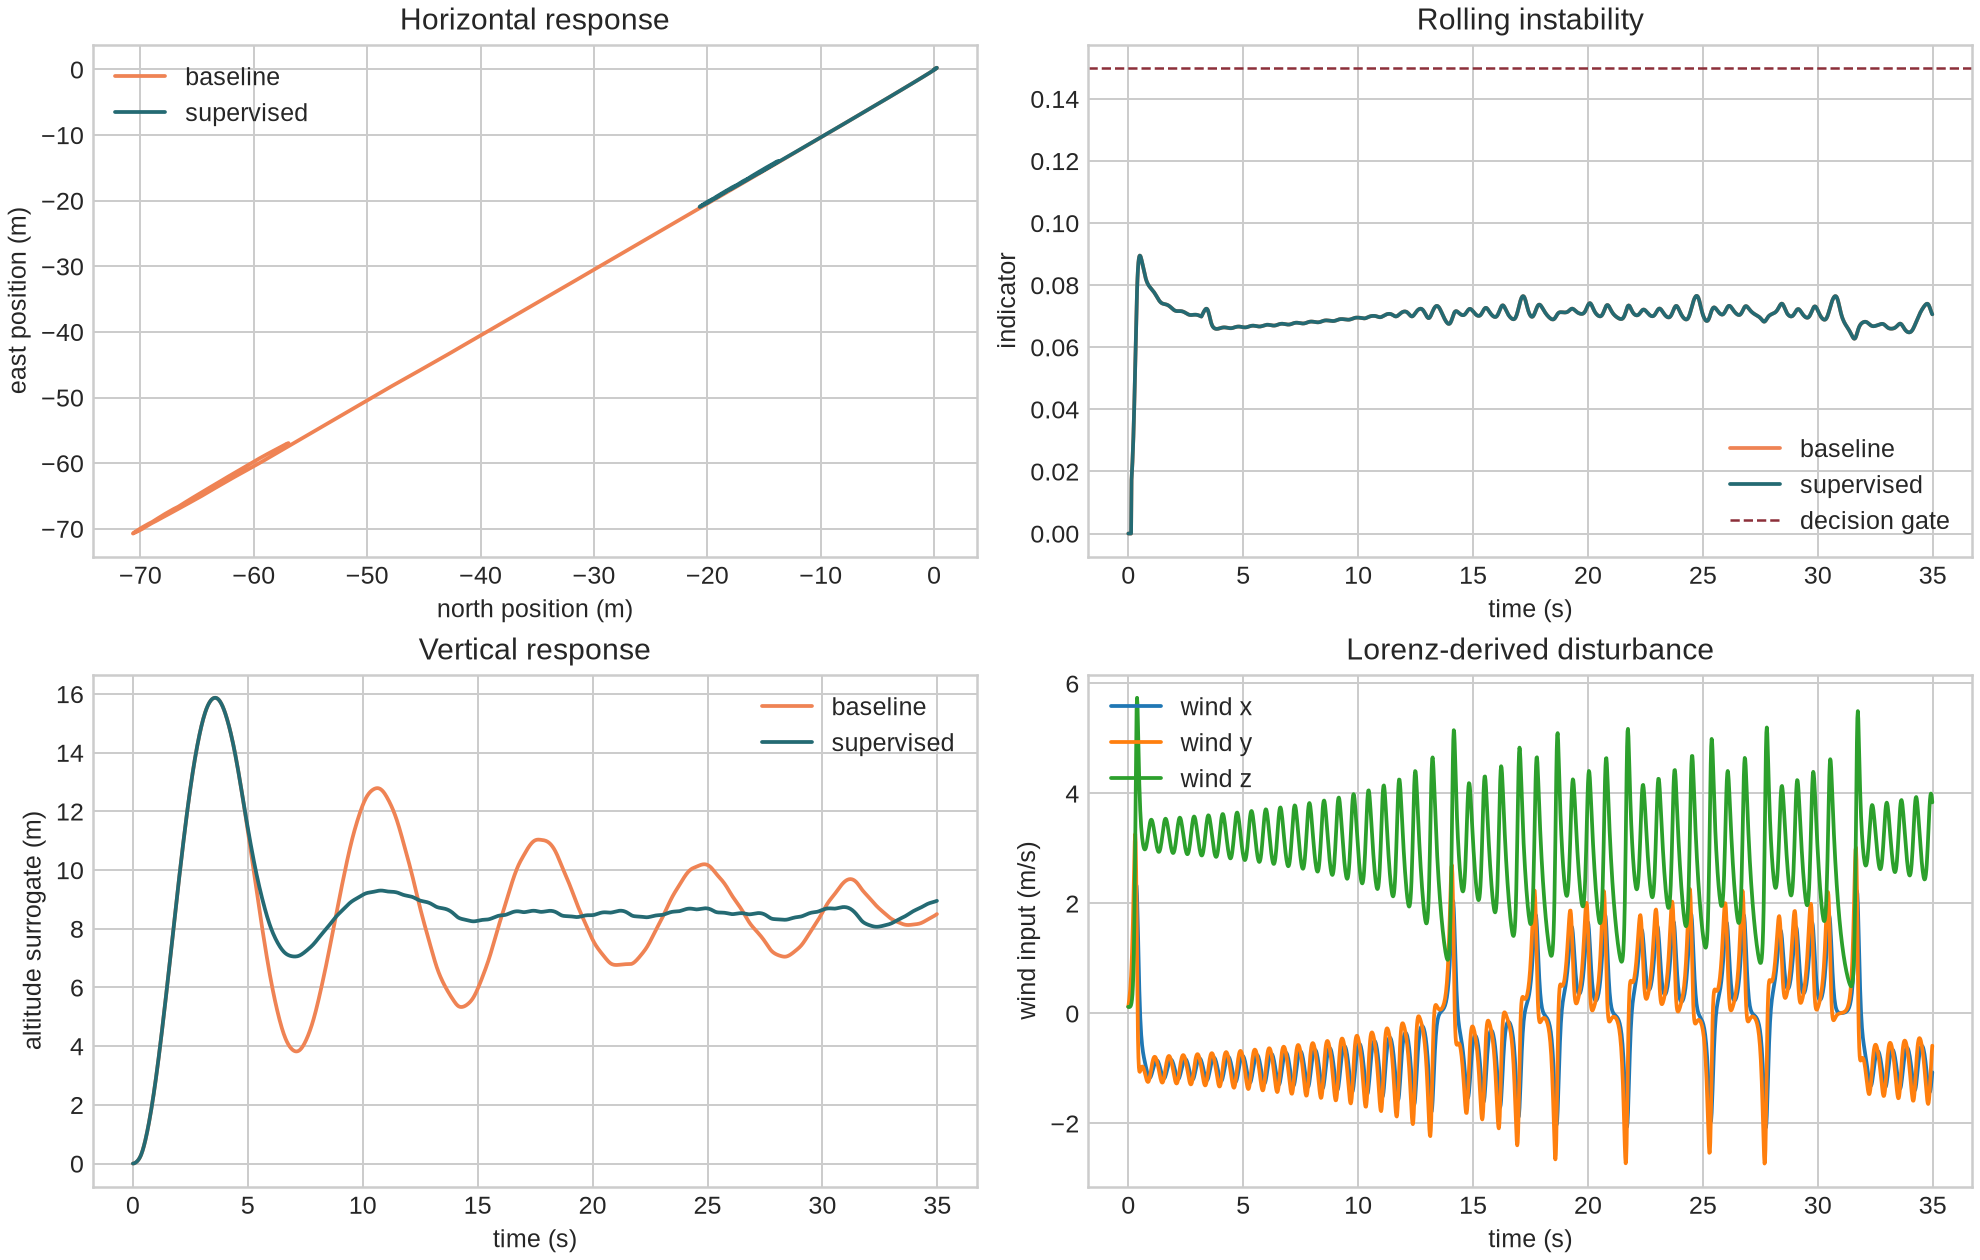
\includegraphics[width=\linewidth]{integration_results.png}
\caption{Reference trajectories, instability, altitude, and Lorenz-derived disturbance.}
\label{fig:integration}
\end{figure}

Figure~\ref{fig:integration} shows the complete integration artifact. The
trajectory panel shows the divergence between an always-hold response and the
supervised response. The instability panel shows that the decision threshold
is not crossed by the peak in this particular run, which is consistent with
the observed return-home event being caused by the position-error gate. This
also illustrates why a single chaos metric should not be presented as a full
control policy.

\section{Discussion and limitations}
The reference result supports a limited conclusion: a safety-gated response
policy can reduce error in this deterministic surrogate under matched forcing.
It does not show that the Lyapunov estimate predicts physical flight behavior,
that the return-home rule is optimal, or that language-model reasoning improves
the result. The experiment uses one seed and therefore provides no estimate of
statistical uncertainty. The point-mass update omits aerodynamic drag,
actuator saturation, estimator delay, PX4 control allocation, communication
loss, and realistic sensor bias.

The live path has additional risks. Coordinate conventions must be checked for
local NED and body frames. Offboard transitions, arming state, watchdogs,
geofencing, failsafes, and manual override need independent tests. A generated
Lorenz wind CSV is not evidence that a Gazebo force was applied. A future study
should run multiple seeds, compare several disturbance magnitudes, vary the
embedding and threshold parameters, inject timing loss, and evaluate flight
metrics such as control effort, settling time, collision margin, and failsafe
response. Physical deployment should only follow a separate safety review.

\section{Conclusion}
This project implements a reproducible supervisory boundary for disturbance-aware
UAV experiments. It combines a bounded telemetry feature, a deterministic
policy, and a locally validated optional LLM proposal without allowing the
remote component to bypass safety checks. In the matched reference experiment,
supervision reduced horizontal RMS and maximum error by about 70 percent. The
result is a software integration finding, not a flight-safety claim.

\section*{Individual member contributions}
\small
\begin{tabularx}{\linewidth}{@{}l X@{}}
\toprule
Name & Contribution \\
\midrule
Shubham Bhilare & Software architecture, Lorenz and telemetry pipeline, safety-gated supervisor, experiments, tests, and reproducibility artifacts. \\
Kadapa Dileep Hussain & Mechanical-systems perspective, UAV disturbance assumptions, experiment review, and interpretation of the flight-related limitations. \\
Dr. Tirtharaj Dash & Research supervision, technical review, evaluation of the AI framing, and final report review. \\
\bottomrule
\end{tabularx}

\smallskip
\noindent All members have read this report and agree with the statement above.

\section*{Generative AI disclosure}
An OpenAI language model was used as a software and writing assistant for
organizing this report, reviewing code, and checking LaTeX compilation. The
language model was not used as the source of the reported numerical results.
All code, experiment outputs, claims, and final text were checked by the
author, who takes responsibility for the submitted work. The optional LLM
interface described in Section 3 is part of the research system and is kept
behind deterministic validation.

\section*{Code availability}
Code, paper source, compiled PDF, figure, tests, and reproduction instructions
are available at:\\
\url{\githuburl}

\begin{thebibliography}{9}
\small
\bibitem{lorenz}
E.~N. Lorenz.
\newblock Deterministic nonperiodic flow.
\newblock \emph{Journal of the Atmospheric Sciences}, 20(2):130--141, 1963.

\bibitem{rosenstein}
M.~T. Rosenstein, J.~J. Collins, and C.~J. De Luca.
\newblock A practical method for calculating largest Lyapunov exponents from
small data sets.
\newblock \emph{Physica D}, 65:117--134, 1993.

\bibitem{russell2021aima}
S.~Russell and P.~Norvig.
\newblock \emph{Artificial Intelligence: A Modern Approach}, 4th edition.
\newblock Pearson, 2021.

\bibitem{px4}
PX4 Development Team.
\newblock PX4 ROS 2 user guide.
\newblock \url{https://docs.px4.io/main/en/ros/}, accessed 2026.

\bibitem{repository}
S.~Bhilare.
\newblock Chaoshawk: UAV chaos-metric supervisor research repository.
\newblock \url{\githuburl}, 2026.
\end{thebibliography}

\end{document}
